% $Id$

\chapter{Removing confounds: a classification example}
\label{sec:confounds_clas}
\minitoc

\section{Introduction}

This chapter describes the steps necessary to remove confounding effects using PRoNTo. Age, gender or scanner/site (in case of a multi-site study) are examples of potential confounds (or covariates) that can be removed from the pattern regression analysis. Please see section \ref{sec:Covariates} for important considerations on covariates.
\\

The dataset used in this chapter can be found on the OASIS's website \url{http://www.oasis-brains.org} (data set 1). In this example, 100 subjects were selected from the OASIS dataset with 50 demented patients and 50 nondemented subjects. Age and gender are considered confounds. Gender is a categorical variable, so it was represented using one-hot encoding (i.e. male was represented as [0 1] and female was represented as [1 0]). The preprocessed data can be found on PRoNTo's website.
\\

We will use PRoNTo to classify subjects with dementia from healthy subjects based on structural MRI scans. We will use Multiple Kernel Learning to classify the subjects based on whole brain images, so the reader is advised to complete the tutorial in Chapter \ref{sec:Block_design_fMRI_dataset} and Chapter \ref{data_example3} before moving on.
\\
 
As in previous Chapters, we will start analyzing the data with PRoNTo's GUI and then repeat the analysis using the {\tt matlabbatch}  system. Please create a folder on your computer to store the results and type {\tt prt} in \matlab{}.

\section{GUI analysis}

\subsection{Data \& Design}

\begin{itemize}
	
	\item In PRoNTo's main window, click on `Data \& Design' and a new window will open, `Data and design'. Like in previous chapters, browse the directory in which to save the PRT structure (saved as `PRT.mat'). 
	
	\item In the panel ‘Groups’, click on `Add’ and provide a name to the group, e.g. `Dem'. We will first add all the information about the demented subjects.
	
	\item All the images in the dataset correspond to different subjects; therefore, click on the ‘Samples’ tick box. This will lock the ‘Subjects/Samples’ field, please see Chapter \ref{sec:SelectBySection} of the manual for more information on this option.
	
	\item In the `Modalities' panel, click on `Add' and provide a name to the modality, e.g. `MRI\_GM', where we used gray matter images.
	
	\item In the `Data format' choose the appropriate format for your data (here nifti); For other data formats the reader is referred to the tutorial of chapter \ref{sec:multimodal_face}.
	
	
	\item Load all the image files belonging to the first group. You can select all the files by using the right mouse button and clicking on the option `Select All', or clicking on the first subject then Shift-click on the last. Please ensure that the order of the images in the selection is as expected (SPM file selector sorts the files based on their names, which can lead to `Scan10' being selected before `Scan2'). When all the images are selected, click on the `Done' button.
	
	\item You can see that the `Design' section is unavailable. Since each subject has only 1 sample/scan, there is no design.
	
	\item Leave the `Regression targets' as it is, i.e `No targets'.
	
	\item In the `Covariates' field, type the covariates you want to regress out. Alternatively, you can save all the covariates in a matrix named {\tt R} and input the full path of this matrix to `Covariates'. Each covariate should be stored in one (continuous confound) or multiple (one-hot encoded categorical confound) columns, hence if there is only one continuous covariate, {\tt R} is a column vector; if there are multiple and/or categorical confounds, {\tt R} will be a matrix containing multiple columns. In this example, we input the full path of a matrix where gender and age are the chosen confounding factors (Figure \ref{fig:confounds_gui_data_and_design_cov}). The file containing matrix R (Dem\_cov.mat) can be found together with the pre-processed OASIS data on PRoNTo's website.
	
	\begin{figure}[!h]
	\centering
		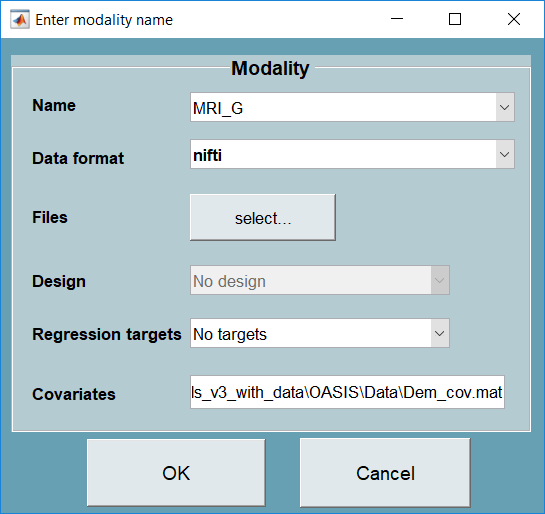
\includegraphics[scale=0.6]{images/Tutorial/v3/confounds/confounds_gui_data_and_design_cov.png}
	\caption{`Specify modality' GUI allows one to enter the covariates to be regressed out.}
	\label{fig:confounds_gui_data_and_design_cov}
	\end{figure}
	
	\item In the `Masks' field, on the bottom left of the `Data and design’ window, select the `mask\_GM' mask (found on OASIS/Data) for the modality specified.
	
	
	\item Finally, repeat the previous steps for a new group, the non-demented group, 'NonDem', including the corresponding images and covariates, and using the same modality and mask as for the `Dem' group. Click on the `Save' button to create the `PRT.mat' file. Notice that the only difference with the tutorials of the previous Chapters is that now we have two groups instead of one (Figure \ref{fig:confounds_gui_data_and_design_review}. The `Data and design' window should look similar to Figure \ref{fig:confounds_gui_data_and_design_final}.
	
\begin{figure}[!h]
\centering
	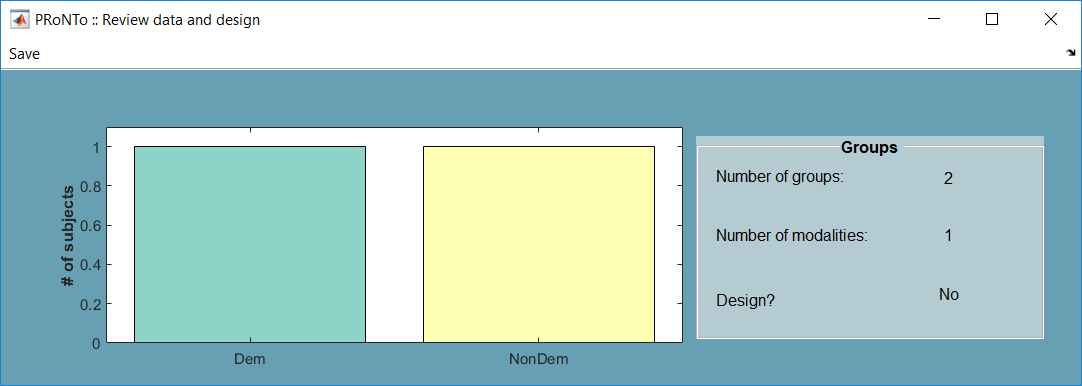
\includegraphics[scale=0.5]{images/Tutorial/v3/confounds/confounds_gui_data_and_design_review.png}
\caption{Review data in the `Data and design' GUI.}
\label{fig:confounds_gui_data_and_design_review}
\end{figure}

\begin{figure}[!h]
\centering
	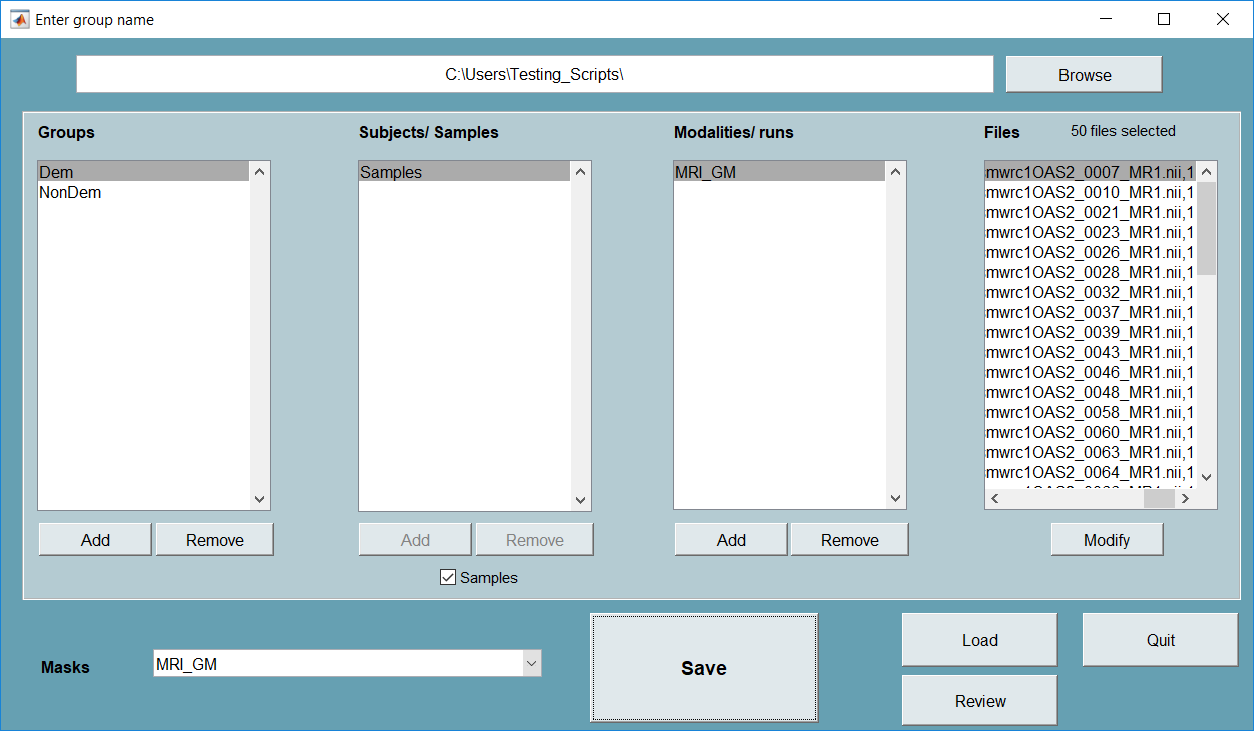
\includegraphics[scale=0.55]{images/Tutorial/v3/confounds/confounds_gui_data_and_design_final.png}
\caption{`Data and design' GUI final configuration.}
\label{fig:confounds_gui_data_and_design_final}
\end{figure}

\end{itemize}

	If no errors are shown in the \matlab{} command, leave the `Data and design' window by clicking `Quit'.
	
%--------------------------------------------------------

\subsection{Prepare feature set}

\begin{itemize}
	
	\item In PRoNTo's main window, click on `Prepare feature set' and a new window will open, `Prepare feature set'.
	
	\item Select the `PRT.mat' file previously created in the `Data \& Design' step and another window will open, `Specify modality to include'. Select the `Build one kernel per region' tick box and load the `AAL' atlas (named `aal\_79x91x69') available in the PRoNTo directory (PRoNTo/atlas/). Leave all the other default options and click `Done'.
		
	\item This will bring you back to the `Prepare feature set' window. Provide a name for the feature set, e.g. `OASIS\_ConfEffects\_withCov'.

	\item Click `Build kernel/data matrix' to build the feature set and kernel.

\end{itemize}


%---------------------------------------------------------------------

\subsection{Model: Specify new}

\begin{itemize}
	
	\item In PRoNTo's main window, click on `Specify new' and a new window will open (see Figure \ref{fig:gui_specify_new} in Chapter \ref{sec:Block_design_fMRI_dataset}).

	\item Select the `PRT.mat' file and provide a name to the model, e.g. `mkl\_OASIS\_ConfEffects\_withCov'.
	
		\item Select one of the `Feature Set' previously defined. In this case, there is only one:  `OASIS\_ConfEffects\_withCov'.
		
	\item Leave the option `Use kernels' tick box as it is, i.e. `Yes'.
	
	\item	Select the `Classification' model type and click on the `Define classes` button. A new window will open, `Specify classes', to define the number of classes and a name for each class. We will define 2 classes. For `Class 1' select group `Dem', and all subjects in this first group and, similarly, for `Class 2' select group `NonDem' and all the subjects in this group. The class names can be any names the user prefers (in alphanumeric characters). Here we simply use the same names as the group names.  Leave the `Subsample according to smallest class' as it is for now. Once you have appropriately specified everything, click `Done'. The final configuration of the `Specify classes' window should look similer to Figure \ref{fig:confounds_gui_specify_model_new_specify_classes}
	
\begin{figure}[!h]
	\centering
		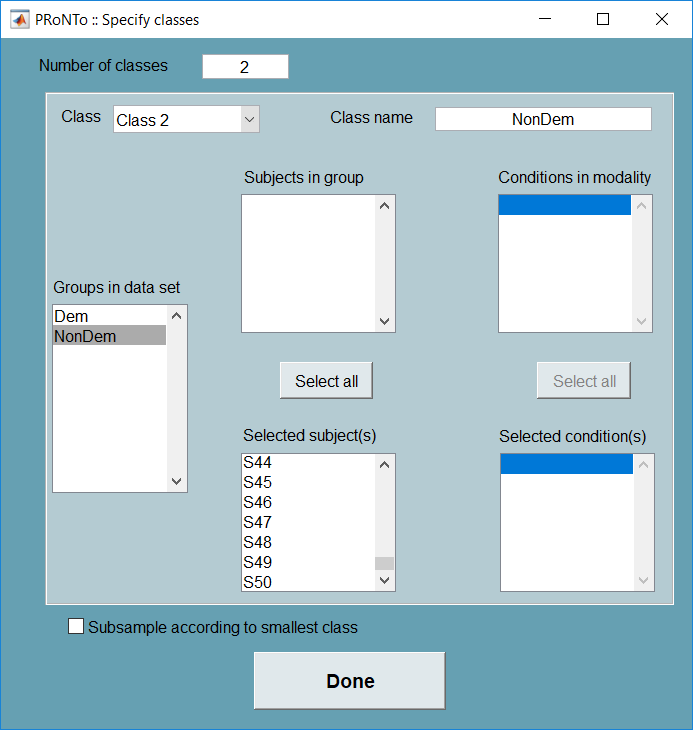
\includegraphics[scale=0.6]{images/Tutorial/v3/confounds/confounds_gui_specify_model_new_specify_classes.png}
	\caption{`Specify classes' GUI.}
	\label{fig:confounds_gui_specify_model_new_specify_classes}
\end{figure}
	
	\item Select the `L1 Multi-Kernel Learning' option, in the `Machine' field.
	
	\item Click the `Optimize hyper-parameter' tick box and leave the range unspecified, i.e. use the default hyper-parameter range. Choose `k-folds CV on Subject per Class' for the `Cross-Validation Scheme' (internal loop), and input 5 in the pop up window defining the number of folds. 
	
	\item Similar to the inner loop, select the `k-folds CV on Subject per Class' cross-validation scheme for the external loop, where k=10.
	
	\item In the `Data operations' box, select the `Mean centre features using training data', `{\color{black}Normalize samples/kernels'} and `Regress out covariates (subject level)' option. The `Regress out covariates (subject level)' option corresponds to the "regressing out" effect of confounds from the data. Note that the order of the operations is important and can affect the results. However, when selected, the `Regress out covariates' option will be performed first (even if not selected as first). Then, the `Specify model' window should look similar to (Figure \ref{fig:confounds_gui_specify_model_new_final}). Click on the `Specify and run model' button.
	
	\item Remember that if you want to check the statistical significance of the results you should specify your models here and run them using the `Model: Run' module where you will have the option of choosing or not to run permutation tests.
	
	
	\begin{figure}[!h]
	\centering
		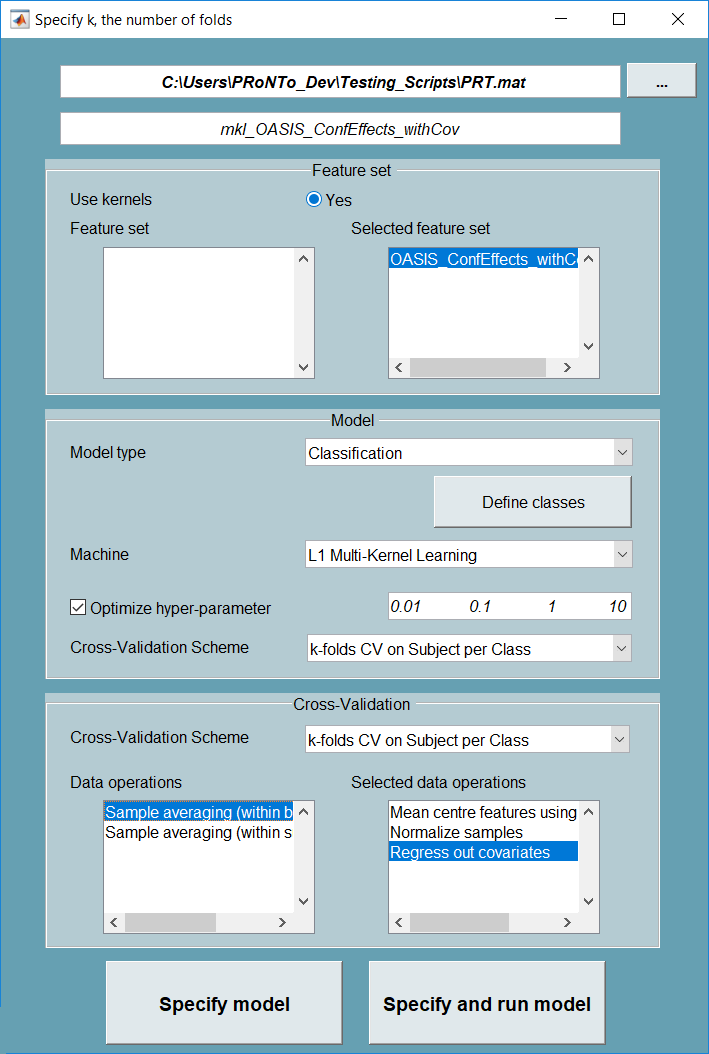
\includegraphics[scale=0.6]{images/Tutorial/v3/confounds/confounds_gui_specify_model_new_final.png}
	\caption{`Specify model' GUI final configuration.}
	\label{fig:confounds_gui_specify_model_new_final}
\end{figure}

	
\end{itemize}

%--------------------------------------------------------------------

\subsection{Model: Specify from}

\begin{itemize}


\item The reader is referred to Chapter \ref{sec:Block_design_fMRI_dataset} and chapter \ref{chap:ModelCrossV} for more details regarding the `Model: Specify from' module.
\end{itemize}
%--------------------------------------------------------------------

\subsection{Model: Run}

The reasons for using the `Model: Run' module and not just click `Specify and run model' in the `Model: Specify new/from' module are the following:

\begin{itemize}
\item One might want to specify one or more models now but run it/them later.
\item One might want to specify more than one models first and run them all together at once afterwards.
\item One might want to run permutation tests in order to check the statistical significance of the results. The reader is referred to Chapter \ref{sec:Block_design_fMRI_dataset} and section \ref{s:DisRes_stats} for more details.

\end{itemize}

%--------------------------------------------------------------------

\subsection{Display results}
\label{display_results_confounds}

\begin{itemize}
	
	\item In PRoNTo's main window, click on `Display results' and select the `PRT.mat' file. This will open the main results window (Figure \ref{fig:confounds_gui_display_results}).
	
\begin{figure}[h!]
	\centering
		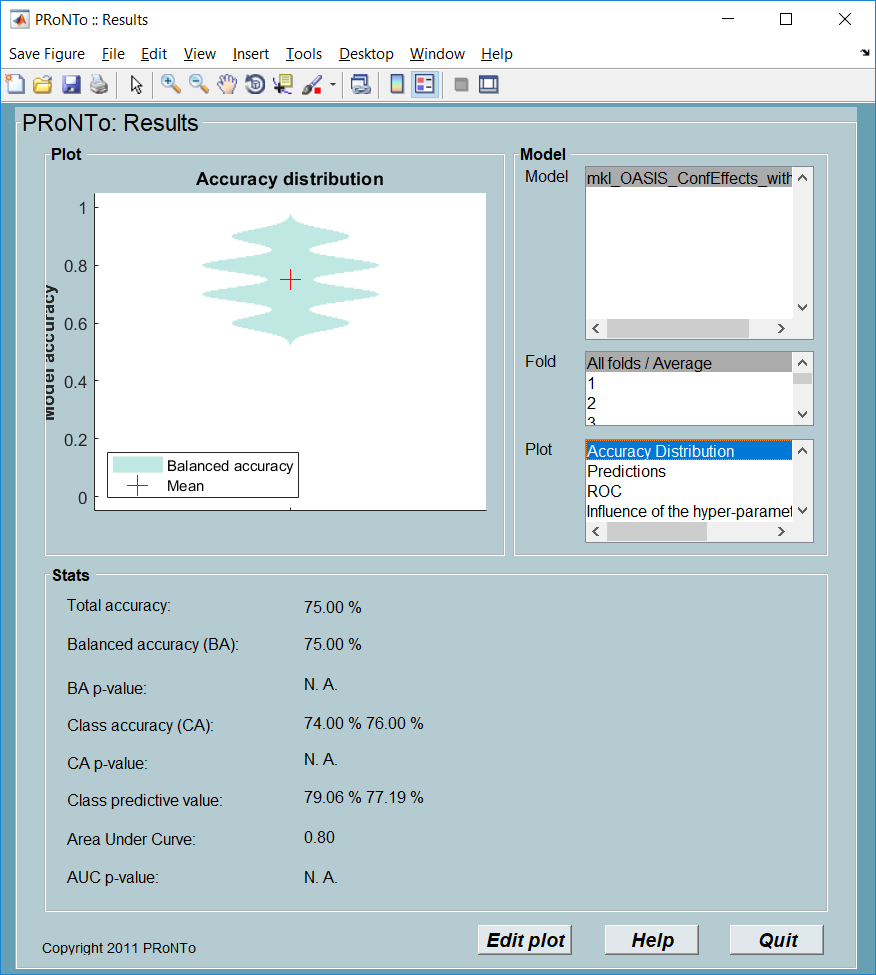
\includegraphics[scale=0.5]{images/Tutorial/v3/confounds/confounds_gui_display_results.png}
	\caption{`Results' GUI.}
	\label{fig:confounds_gui_display_results}
\end{figure}
	
	
	\item In the `Results' window, we have different performance measures, as well as different plots; both the average as well as for each fold. One can select different plots in the `Plots' list. For further information regarding the `Display results' module the reader is referred to chapter \ref{chap:DisRes}.

\end{itemize}

%=====================================================

\section{Batch analysis}
\label{sec:Batch_analysis_svm_confounds}

In this section, the previous experiment will be repeated using the `\texttt{matlabbatch}' system. The reader is advised to complete the tutorial in Section \ref{sec:Batch_analysis_svm} before continuing, since the explanation of each step will be less detailed.

Once again, to analyse the data, create a new directory to save the results of the analysis. On the main interface of PRoNTo click on the `Batch' button to open the `{\tt matlabbatch}'. Alternatively, type `prt\_batch' in the \matlab{}  prompt.

%--------------------------------------------------------------

\subsection{Data \& Design}

\begin{itemize}

 	\item Click on `Data \& Design' in the PRoNTo menu.
 	
	\item In the `Directory' field, select a directory where the `PRT.mat' file will be saved.
	
	\item In the `Groups' field:
 	
		\begin{itemize}
		
		\item Add two groups.
		
		\item In the field `Name', provide a name without spaces to both groups, e.g. `Dem' and 'NonDem'. 
		
		\item In the field `Select by', select the `Samples' option and add a new modality. For more information on the Samples option please refer to chapter \ref{chap:DataDesign}.
		
		\item For both groups add one modality and provide the same name, e.g. `MRI\_GM'.
		
		\item For both groups select `nifti' for our data format.
		
		\item In the field `Files', select the proper images for each of the groups.	
		
		\item For both groups leave the `Regression targets (subject)' as it is, i.e. `No targets'.
		
		\item Specify as `Covariates' the file with the confounds you want to remove. Remember that this file should contain a variable `R' with a matrix of covariates.
	
	\end{itemize}
	
	\item In the `Masks' field, add a new modality, provide the same modality name, `MRI\_GM'; choose the appropriate data format and select the `mask\_GM' mask available in the Oasis dataset. The name of the modality here has to be exactly the same as in `Modalities'.
	
	\item Leave the `HRF overlap' and the `HRF delay' fields as default.
	
	\item In the `Review' field, select `Yes' if you would like to review your data and design in a separate window. Otherwise, leave as it is, i.e. `No'. Note: if `Yes' is selected, users will need to close the Review window after Running the batch to allow the execution of following modules.

\end{itemize}

The final configuration of the {\tt matlabbatch} `Data \& Design' module should look similar to Figure \ref{fig:confounds_batch_data_and_design_final}.

		\begin{figure}[h!]
	\centering
		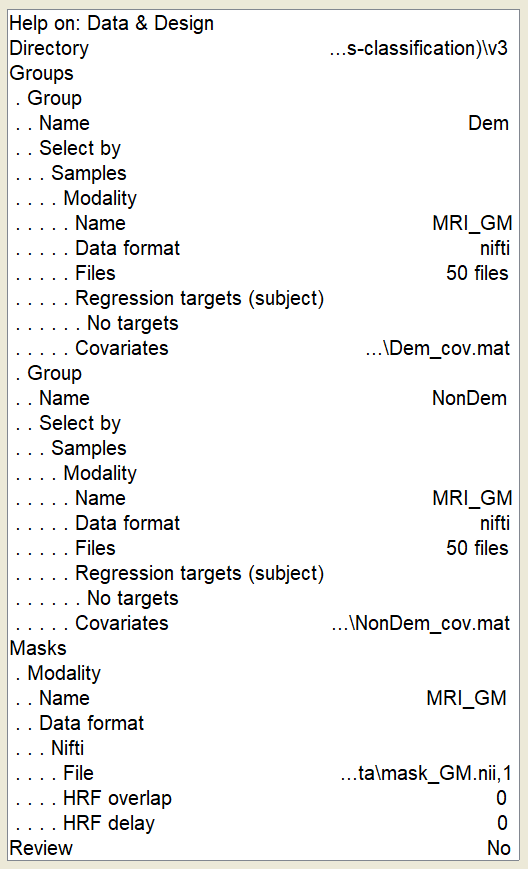
\includegraphics[scale=0.6]{images/Tutorial/v3/confounds/confounds_batch_data_and_design_final.png}
	\caption{`Data \& Design' module in {\tt matlabbatch}. }
	\label{fig:confounds_batch_data_and_design_final}
	\end{figure}

The batch can either be run directly or the following modules can be added to complete multiple steps of the analysis at once. We typically suggest users to save and run the `Data and Design' step in a separate batch to avoid deleting/overwriting the {\tt PRT} each time the batch is run.

%------------------------------------------------------------

\subsection{Feature set / Kernel}

\begin{itemize}
	\item Click on the `Feature set / Kernel' option on PRoNTo's {\tt matlabbatch} menu.
	
	\item With `Load PRT.mat' field selected, click on the `Dependency' button to associate the `PRT.mat' file created in the previous `Data \& Design' step or click on the `Select files' button to browse where `PRT.mat' file was saved. The window of Figure \ref{fig:batch_feature_set_dep} in Chapter \ref{sec:Block_design_fMRI_dataset} is called to establish a dependency connection with the previous `Data \& design' module.
	
	
    \item Provide a name for the `Feature set/kernel', e.g. `OASIS\_ConfEffects\_withCov'.
	
	\item Choose the appropriate data format, add one modality and select the modality name with the `Dependency' button\footnote{Or type it in manually, `MRI\_GM', but the name needs to be {\it exactly} the same as the one specified in the `Data \& Design' module.}(Data \& Design:Mod\#1 name).
	
		\begin{itemize}
	
	\item In the `Samples/Conditions' field , select the `All samples' option.
	
	\item In the `Voxels to include' field, select `All voxels' option, this means we are not entering an additional second-level mask.
	
	\item In the `Detrend' field, select `None'.
	
	\item In the `Scale input scans' field, select the `No scaling' option.
	
	\item And finally in the `Use atlas to build ROI specific kernels' field, load the AAL atlas as we did in the GUI section. After all these steps, the batch editor should look similar to the one in Figure \ref{fig:confounds_batch_prepare_featureSet_final}.
	
	\begin{figure}[h!]
	\centering
		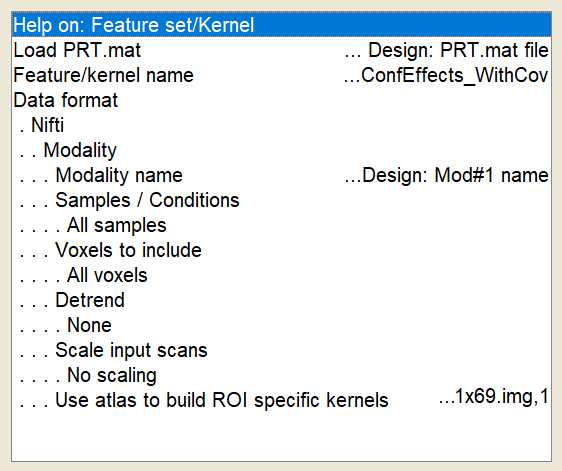
\includegraphics[scale=0.6]{images/Tutorial/v3/confounds/confounds_batch_prepare_featureSet_final.png}
	\caption{Final configuration of the {\tt matlabbatch} `Feature set / Kernel' module.}
	\label{fig:confounds_batch_prepare_featureSet_final}
\end{figure}
	
	\end{itemize}

\end{itemize}

%--------------------------------------------------------

\subsection{Model: Specify new}

\begin{itemize}

\item Click on the `Model: Specify new' option on PRoNTo's {\tt matlabbatch} menu.
	
\item With `Load PRT.mat' field selected, click on the `Dependency' button to associate the `PRT.mat' file created in the previous `Feature set / Kernel' step or click on the `Select files' button to browse where `PRT.mat' file was saved.

\item Provide a name for the model, e.g. `mkl\_OASIS\_ConfEffects\_withCov'.   

\item In the `Feature sets' field, select the feature set name with the `Dependency' button\footnote{or write it {\it exactly} as previously defined in the `Feature set / Kernel' module (option `Feature set/Kernel: Feature/kernel name'), here `OASIS\_ConfEffects\_withCov'.}.
	
	\item Select the `Classification' model type:
	
		\begin{itemize}
		
		\item Add 2 new classes.
		
		\item For Class (1), specify a name by writing `Dem' or using Dependency to choose the first group's name defined in 'Data \& Design' and add one group. The class name doesn't have to be the same as the group name, this example uses this only for simplicity. After this step, select the group name from the `Data \& Design' module (`Data \& Design:Group\#1 name') with the `Dependency' button\footnote{Or write it {\it exactly}, as previously defined in the Data \& Design' module, here `Dem'}.
		
		\item In the `Subjects' field of Group 1, type `1:50'. This will tell the program to use all the 50 subjects, i.e. from subject 1 to scan 50. In Conditions/Samples, select `All Samples'. 
		
		\item Similar to Class (1),  write `NonDem' on the name field for Class (2), or use Dependency to choose the second group's name. Then fill the group name using Dependency, i.e. the second group's name created in the `Data \& Design' module, `NonDem'. In the `Subjects' field of Group 2, type `1:50'. In Conditions/Scans, select `All scans'. 
		
		\item Finally leave `Subsample example based on class definition' as it is, i.e. `No'.

		\end{itemize}			
		
	\item In the `Machine' field:
	
	\begin{itemize}
	
	\item Select `Kernel machine' and the `L1 Multi-Kernel Learning' option.	
	
	\item In the `Machine optimization and parameters' select the `Optimize hyper-parameter' and leave it to the default values (i.e. `10\^{}[-2:3]').
	
	\item In the `Cross validation type for hyper-parameter optimization' field, choose `k-folds CV on subjects per group', and input `5' in the field `k'.  
	
	
	\end{itemize}
	
	\item In the `Cross-validation type' field, choose `k-folds CV on subjects per group', and input `10' in the field `k'.
	
	\item Leave the `Include all scans' field as it is, i.e. `No'.

	\item In the `Data operations' field:
	
		\begin{itemize}
		\item  Leave the `Mean centre features' field as it is, i.e. `Yes'. 
				
		\item  Click on the `Other Operations' button, choose `Select operations', `New Operation' and select the `{\color{black}Normalize samples/kernels'}. 
		
		\item Click `Select operations', `New Operation', and select `Regress out covariates (subject level)' option from the list. 
		\end{itemize}
\end{itemize}

After these steps, the batch editor should look similar to the one in Figure \ref{fig:confounds_batch_model_specify_new_final}.	

\begin{figure}[h!]
\centering
	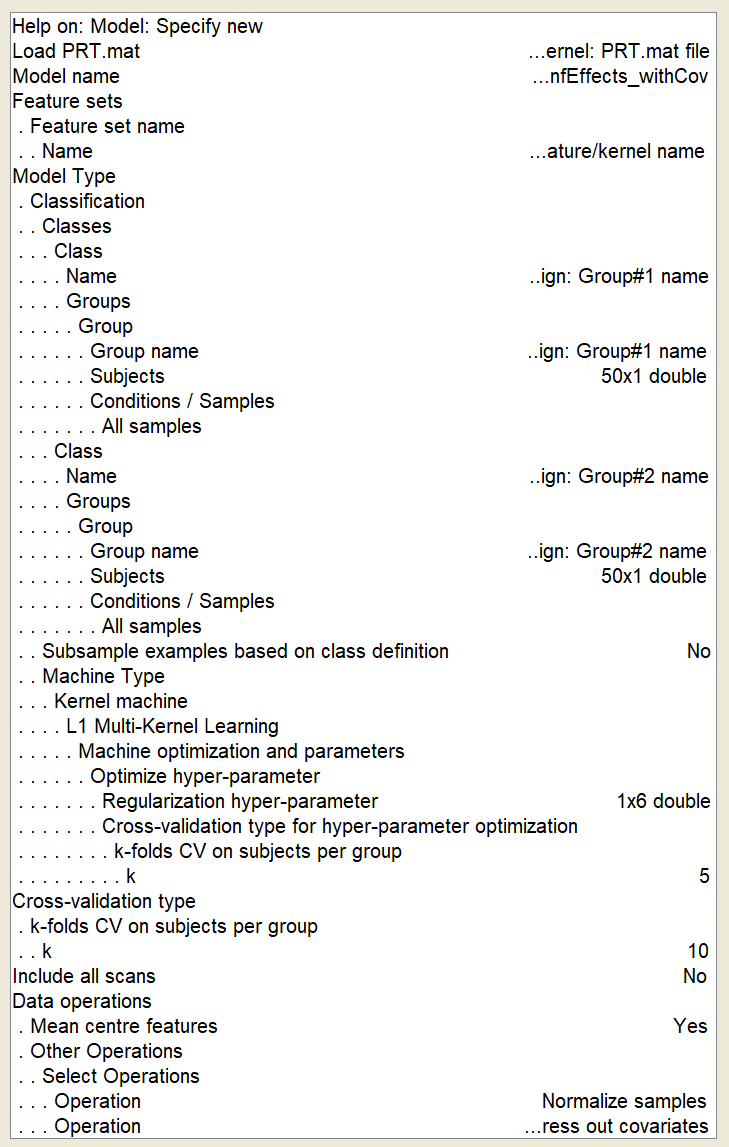
\includegraphics[scale=0.6]{images/Tutorial/v3/confounds/confounds_batch_model_specify_new_final.png}
\caption{Final configuration of the {\tt matlabbatch} `Model: Specify new' module.}
\label{fig:confounds_batch_model_specify_new_final}
\end{figure}

%----------------------------------------------------------

\subsection{Model: Run}

\begin{itemize}

    \item Click on the `Model: Run' option in PRoNTo's {\tt matlabbatch} menu.
    
   	\item  With the `Load PRT.mat' field selected, click on the `Dependency' button to associate the `PRT.mat' file updated in the previous `Specify model' step.

    \item Select the model name from the `Specify model' module with the `Dependency' button\footnote{or write it {\it exactly} as previously defined in the `Specify model' module, here `mkl\_OASIS\_ConfEffects\_withCov'}.
    
    \item In the field `Do permutation test?', leave as it is, i.e. `No permutation test'. 

\end{itemize}

%----------------------------------------------------------
\subsection{Compute weights}
\begin{itemize}

\item Click on the `Compute weights' option in PRoNTo's {\tt matlabbatch} menu.

\item With the `Load PRT.mat' field selected, click on the `Dependency' button to associate the `PRT.mat' file updated in the previous `Run model' step.

\item In the `Model name' field, click on the `Dependency' button to associate the model name from the `Specify model' module.

\item In `Build weight images per ROI', users can choose `Load atlas' to build a weight image showing where the value in each region corresponds to the region/kernel's weight. This example uses MKL, where the AAL atlas was selected during the Feature set module, hence the atlas will be automatically loaded here if `Load atlas' is selected.  

\item Leave the other fields as default.

\end{itemize}

We are now ready to run the batch: the arrow on top of the {\tt matlabbatch} should be green and can be clicked. If the arrow is gray, please check for missing inputs in the different modules (displayed with an `$<--$X').


%----------------------------------------------------------


\subsection{Display weights}

\begin{itemize}
	
	\item In PRoNTo's main window, click on `Display weights' and select the `PRT.mat' file. This will open the `PRoNTo::Weights' window.
	
	\item In the Display panel, click the model name in the `Model' field, `mkl\_OASIS\_ConfEffects\_withCov'. An image will appear in the `Weights map' panel. To show the `Anatomical img' you have to load an anatomical image for reference. A template image can be found in SPM's canonical folder (`single\_subj\_T1` file). Select `weights per region' to display the kernel/ROI contributions (see Chapter \ref{chap:ComputeWeights} for details on this image). Select `weights per voxel' to display the voxels contributions. In the table below the weight map, the contribution of ROI to the model and its corresponding rank are listed. A bar graph shows the contribution of each ROI to the model (sorted), displaying how `sparse' the model is. The final window will look similar to the one shown in the Figure \ref{fig:confounds_batch_display_weights}.
	
\begin{figure}[h!]
\centering
	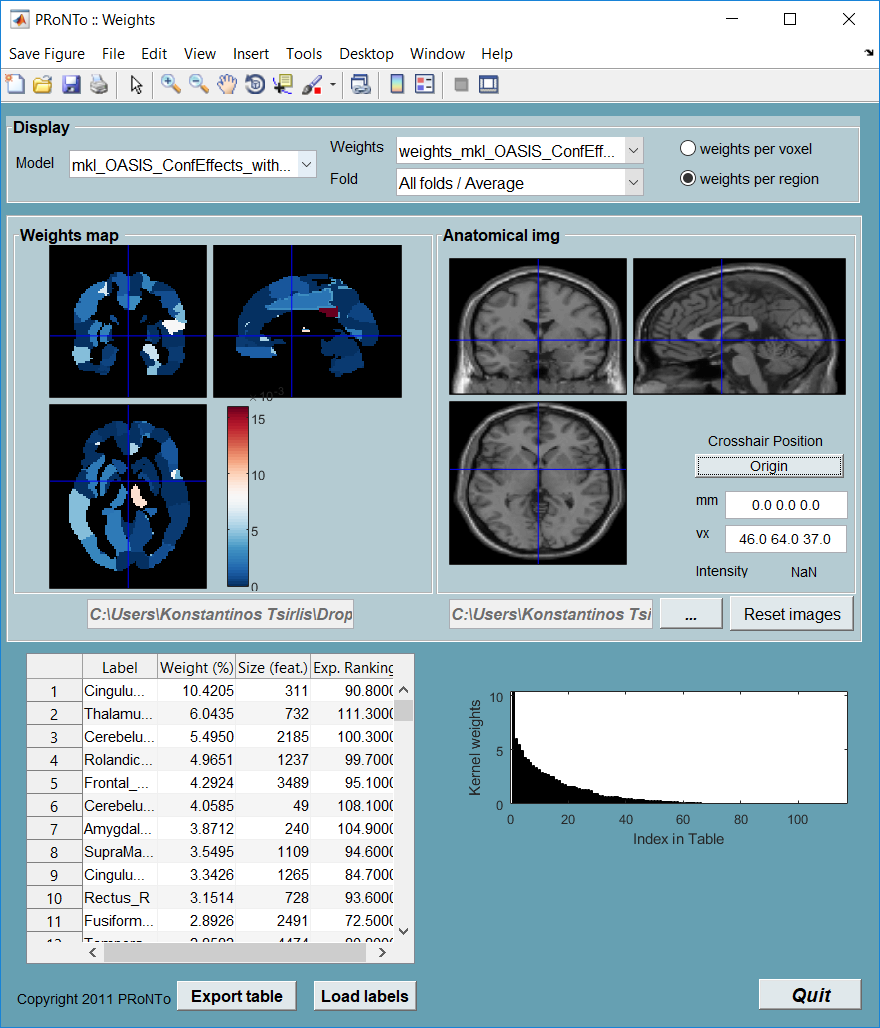
\includegraphics[scale=0.45]{images/Tutorial/v3/confounds/confounds_batch_display_weights.png}
\caption{`Display weights' module where a weight map per region is shown.}
\label{fig:confounds_batch_display_weights}
\end{figure}

	
\end{itemize}


%-----------------------------------------------------------------------------------


\section{Effects of removing covariates}

This section shows the differences between results with and without removing covariates.\\

In order to check the effects of regressing out covariates one has to rerun the whole procedure keeping everything the same, except that now we have to not choose `Regress out covariates' in the `Data operations' when we specify our new model. This can be more easily done using the module `Model: Specify from'. %%%%%% ADD A MODEL:SPECIFY FROM FIGURE !!!!

Figure \ref{fig:confounds_batch_display_results_without_regress} shows the accuracy of the same MKL model but without removing confounds: the average balanced accuracy decreased from 75\% (see \ref{fig:confounds_gui_display_results}) to 64\%.

\begin{figure}[!h]
	\centering
	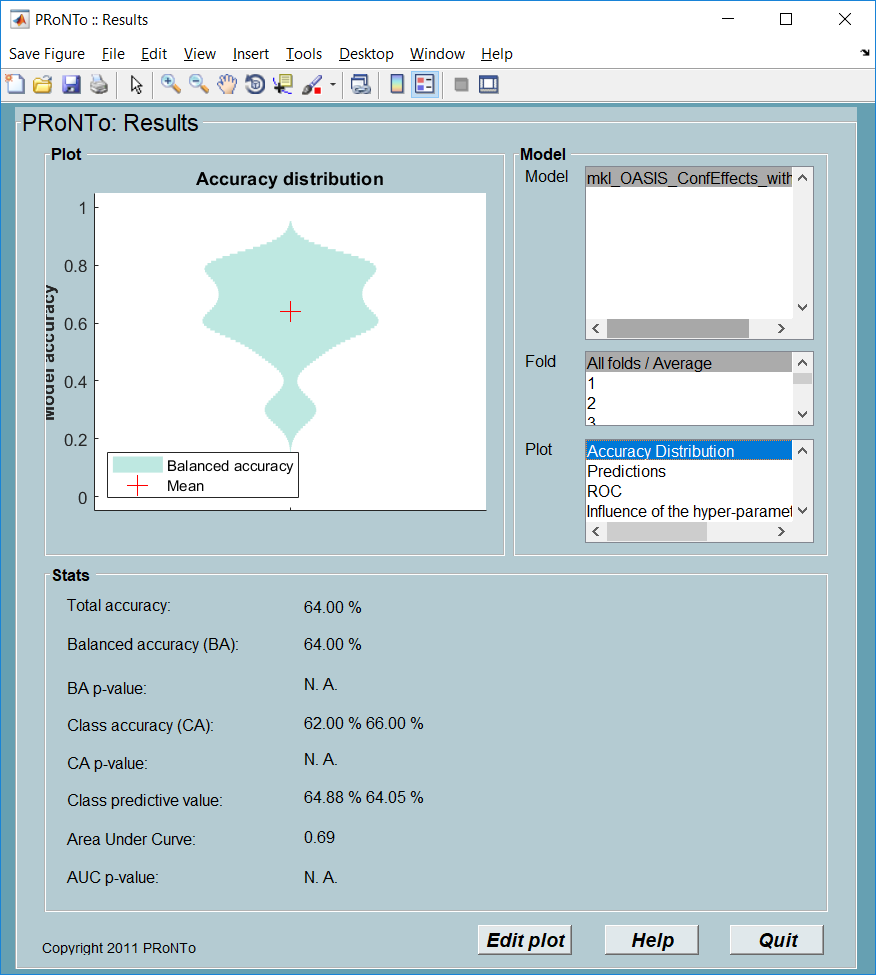
\includegraphics[scale=0.47]{images/Tutorial/v3/confounds/confounds_batch_display_results_without_regress.png}
	\caption{`Display results' GUI with the accuracies of MKL without removing covariates.}
	\label{fig:confounds_batch_display_results_without_regress}
\end{figure}







